% =====================================================================
%  RDT-UnB — Relatório final (Entregas 1, 2 e 3) — CIC0236 TR2 2026/2
%  Limite: 15 páginas. Todos os números vêm da campanha de 15/11/2026
%  (results/final no repositório).
% =====================================================================
\documentclass[11pt,a4paper]{article}

\usepackage[T1]{fontenc}
\usepackage[utf8]{inputenc}
\usepackage[brazil]{babel}
\usepackage{lmodern}
\usepackage[a4paper,margin=2.2cm]{geometry}
\usepackage{amsmath,amssymb}
\usepackage{graphicx}
\usepackage{booktabs}
\usepackage{array}
\usepackage{float}
\usepackage{subcaption}
\usepackage{xcolor}
\usepackage{enumitem}
\usepackage[hidelinks]{hyperref}
\hypersetup{colorlinks=true,linkcolor=blue,citecolor=blue,urlcolor=blue}
\setlength{\emergencystretch}{3em}

\addto\captionsbrazil{\renewcommand{\refname}{Referências bibliográficas}}

\newcommand{\pend}[1]{\textcolor{red}{[#1]}}

\newcommand{\figura}[4]{%
  \begin{figure}[H]
    \centering
    \includegraphics[width=#2]{#1}
    \caption{#3}
    \label{#4}
  \end{figure}}

\begin{document}

% ======================= CAPA ========================================
\begin{titlepage}
  \centering
  \IfFileExists{../imgs/logo_unb.png}{
\includegraphics[width=0.22\textwidth]{../imgs/logo_unb.png}\\[0.6em]}{}
  {\large\textbf{Universidade de Brasília}}\\
  Departamento de Ciência da Computação\\
  CIC0236 Teleinformática e Redes 2

  \vfill
  {\LARGE\textbf{RDT-UnB: relatório final}}\\[0.8em]
  {\large Evolução de SAW a protocolos de janela com RTT adaptativo}
  \vfill

  \begin{tabular}{ll}
    231013510 & Atila Sousa Fernandes\\
    231013645 & Lucas Adeodato de Oliveira\\
    222005395 & Lurian Correia Lima
  \end{tabular}

  \vfill
  15 de novembro de 2026
\end{titlepage}

\pagenumbering{roman}
\tableofcontents
\clearpage
\pagenumbering{arabic}

% ======================= 1 ===========================================
\section{Introdução e evolução do projeto}

O servidor do projeto (\texttt{137.131.178.229:8080}) é uma caixa-preta UDP que
só envia um \texttt{DATA} quando recebe um \texttt{REQ}. Sobre ele construímos
um cliente que acrescenta confiabilidade ao UDP~\cite{rfc768} com os mecanismos
das Seções~3.4 e~3.5 de Kurose e Ross~\cite{kurose}: número de sequência, ACK,
temporizador, retransmissão e verificação do arquivo por MD5~\cite{rfc1321}. O
cliente evoluiu em três entregas, e cada uma atacou o gargalo que os dados da
anterior mostraram.

Para este relatório, rodamos de novo todos os experimentos das três entregas
numa única campanha, em 15/11, com o código final e o mesmo timeout fixo de
1000\,ms em todas as comparações. Assim todas as tabelas vêm da mesma rede e do
mesmo arquivo: o MD5 do \emph{large} é o mesmo nas 20 execuções com ele.

\subsection{Entrega 1: Stop-and-Wait}

O cliente SAW faz o handshake \texttt{HELLO}/\texttt{OK}, que negocia o
\texttt{segment\_size} (512\,B) e informa o MD5 do arquivo. Em seguida pede um
segmento por vez (\texttt{REQ} $\to$ \texttt{DATA} $\to$ \texttt{ACK}), com
timeout fixo e até 10 retransmissões, e encerra com
\texttt{FIN|checksum=<md5>} e \texttt{DONE|ok=1}. O \texttt{DATA} é separado
só nas três primeiras barras, porque o payload binário pode conter o byte
\texttt{|}. Cada sessão gera um CSV com uma linha por segmento, com
\emph{timestamps} do relógio do sistema, o mesmo do Wireshark.

O throughput do SAW foi de 140,6\,kbit/s no \emph{small}, 151,5\,kbit/s no
\emph{medium} e 140,9\,kbit/s no \emph{large}, praticamente o limite de um
segmento por RTT ($512 \cdot 8 / 29\text{ ms} \approx 141$\,kbit/s). O CSV mostra
o motivo: a soma dos RTTs ocupa 99,9\% do tempo de cada sessão. O cliente passa quase todo o
tempo esperando o \texttt{DATA} do único \texttt{REQ} em voo. O \emph{medium}
ficou um pouco acima dos outros porque o RTT médio dessa execução foi menor
(26,8\,ms contra 29,0\,ms).

\subsection{Entrega 2: janela deslizante}

Para sair desse limite, implementamos o Go-Back-N (GBN) e o Selective Repeat
(SR), com até $N$ \texttt{REQ}s em voo. No GBN o cliente só aceita o
\texttt{DATA} da base da janela e, quando o timer da base vence, reenvia a
janela inteira. No SR cada segmento tem seu próprio timer, os \texttt{DATA}
fora de ordem ficam num \emph{buffer} e só o segmento atrasado é reenviado.

A perda é simulada no cliente: cada \texttt{DATA} recebido é descartado com
probabilidade $P$ (opção \texttt{--loss}, semente fixa 42). Não simulamos a
perda do \texttt{ACK} porque o servidor não usa o \texttt{ACK}: só a falta do
\texttt{DATA} dispara uma retransmissão. Testamos janelas de 4, 8 e 16 com 0,
5 e 10\% de perda no arquivo \emph{small} (21 cenários).

Sem perda, o SR com $N=16$ chegou a 2\,000,6\,kbit/s no \emph{small}, 14
vezes o SAW (140,6\,kbit/s), e janelas maiores foram sempre mais rápidas. Com
10\% de perda e $N=16$, o SR fez 220 retransmissões, uma por perda simulada,
e terminou em 104\,s. O GBN fez 3\,556, porque cada timeout da base reenvia a
janela inteira, e levou 226\,s. No GBN, aumentar a janela de 4 para 16
quadruplicou as retransmissões (920 para 3\,556) e quase não mudou o tempo
(243 para 226\,s).

Duas dificuldades marcaram essa etapa. GBN e SR foram escritos em branches
separados, e a integração num único cliente exigiu reorganizar a interface de
linha de comando. Depois, um servidor de teste local que embaralhava a ordem
das respostas fez o GBN levar 250\,s em vez de 1\,s sem perda, porque o
receptor GBN descarta todo \texttt{DATA} fora de ordem. O servidor real responde
em ordem, e passamos a testar assim.

\subsection{Entrega 3: RTT adaptativo}

Com perda, o timeout fixo de 1\,s passou a ser o maior custo: cada
\texttt{DATA} perdido deixa o segmento parado por cerca de 30 RTTs. A primeira
versão do timeout adaptativo, só com a fórmula $\text{EstimatedRTT} +
4\,\text{DevRTT}$, gerou mais de mil retransmissões numa transferência sem
nenhuma perda. Com a
rede estável o DevRTT cai perto de zero, o timeout fica colado no RTT e
qualquer atraso de poucos milissegundos dispara um timeout prematuro. A
correção foi um piso no timeout (50\,ms) e o dobro do timeout a cada
retransmissão do mesmo segmento. A Seção~\ref{sec:rtt} detalha as duas
decisões e a escolha de $\alpha$ e $\beta$.

% ======================= 2 ===========================================
\section{RTT adaptativo: implementação}
\label{sec:rtt}

O timeout adaptativo está no SR e é ligado com \texttt{--adaptive}. O GBN
continua com timeout fixo. O cliente funciona assim:
\begin{itemize}[nosep]
  \item Até a primeira amostra vale o timeout inicial de 1000\,ms. Na primeira
    amostra, $\text{EstimatedRTT} = \text{SampleRTT}$ e
    $\text{DevRTT} = \text{SampleRTT}/2$.
  \item O RTT de um segmento é o tempo entre o \texttt{REQ} e o \texttt{DATA}
    correspondente. Só segmentos sem retransmissão geram amostra, como no
    TCP~\cite{kurose}: se o \texttt{REQ} foi repetido, não dá para saber a qual
    dos dois o \texttt{DATA} responde. Nesses segmentos, \texttt{rtt\_ms} fica
    vazio no CSV.
  \item Cada \texttt{REQ} novo usa o timeout corrente, gravado na coluna
    \texttt{timeout\_ms}. A cada retransmissão, o timeout daquele segmento
    dobra, como no TCP (Kurose~\cite{kurose}, Seção~3.5.4).
  \item O servidor responde a todo \texttt{REQ}. Se um segmento foi reenviado
    uma vez e chegam dois \texttt{DATA} dele, o primeiro respondia ao
    \texttt{REQ} original e a retransmissão foi desnecessária. Nesse caso o
    tempo desde o \texttt{REQ} original entra como amostra. Isso não existe no
    TCP; usamos porque, sem essas amostras, o estimador nunca veria os RTTs
    mais altos, que são justamente os que causam timeout.
\end{itemize}

\subsection{Estimativa EWMA}

As fórmulas implementadas são as de Kurose~\cite{kurose}, Seção~3.5.3, com um
piso no timeout:
\begin{equation}
  \text{EstimatedRTT} \leftarrow (1-\alpha)\,\text{EstimatedRTT} + \alpha\,\text{SampleRTT},
\end{equation}
\begin{equation}
  \text{DevRTT} \leftarrow (1-\beta)\,\text{DevRTT} + \beta\,\lvert \text{SampleRTT} - \text{EstimatedRTT}\rvert,
\end{equation}
\begin{equation}
  \text{Timeout} = \max\!\bigl(\text{MinTimeout},\; \text{EstimatedRTT} + 4\,\text{DevRTT}\bigr),
\end{equation}
com $\alpha = 0{,}125$, $\beta = 0{,}25$ e $\text{MinTimeout} = 50$\,ms. O DevRTT
é atualizado com o EstimatedRTT anterior, antes de ele mudar.

\subsection{Piso do timeout}
\label{sec:piso}

Kurose~\cite{kurose} recomenda que o timeout fique acima do EstimatedRTT com uma
margem proporcional à variação do RTT, para evitar retransmissões
desnecessárias; é o papel do termo $4\,\text{DevRTT}$. Na nossa rede essa
margem às vezes some: sem piso, o DevRTT ficou abaixo de 1\,ms em 85\% dos
segmentos, e o primeiro atraso maior estoura o timer. O piso garante uma margem mínima. A
Tabela~\ref{tab:piso} varia só o piso (SR, $N=16$, \emph{large}).

\begin{table}[H]
\centering\small
\begin{tabular}{rrrrr}
\toprule
Perda & Piso (ms) & Tempo (s) & Retransmissões & Desnecessárias \\
\midrule
0\%  & 0$^*$  & 38,6  & 1\,433 & 1\,433 \\
0\%  & 50$^*$ & 40,5  & 29     & 29 \\
0\%  & 100 & 37,0  & 0      & 0 \\
0\%  & 200 & 50,0  & 0      & 0 \\
\midrule
10\% & 0   & 86,8  & 3\,237 & 970 \\
10\% & 50  & 101,4 & 2\,326 & 59 \\
10\% & 100 & 184,3 & 2\,700 & 0 \\
10\% & 200 & 293,6 & 2\,267 & 0 \\
\bottomrule
\end{tabular}
\caption{Efeito do piso do timeout (SR, $N=16$, \emph{large}, $\alpha=0{,}125$,
$\beta=0{,}25$). ``Desnecessárias'' são as retransmissões em que o
\texttt{DATA} original chegou depois do \texttt{REQ} repetido. $^*$Mediana de
3 repetições intercaladas; as demais linhas são uma execução.}
\label{tab:piso}
\end{table}

Com 10\% de perda, que é onde o timeout adaptativo importa, o piso de 50\,ms
foi o melhor compromisso. Sem piso, 970 das 3\,237 retransmissões foram
desnecessárias. Com 100 e 200\,ms quase não há retransmissão desnecessária,
mas cada perda espera mais, e o tempo total sobe para 184 e 294\,s. Com
100\,ms, as 2\,700 retransmissões passam das $\sim$2\,270 perdas simuladas sem
aparecerem como desnecessárias: são segmentos reenviados mais de uma vez, e o
cliente só reconhece a retransmissão desnecessária quando o segmento foi
reenviado uma única vez.

Na campanha, sem perda, o piso 0 teve menos retransmissões que o de 50\,ms
(1\,089 contra 1\,840), o contrário do esperado: sem piso o timeout fica mais
perto do RTT. Como cada linha era uma execução só, não dava para saber se a
diferença vinha do piso ou da rede naquele minuto. Por isso repetimos os dois
pisos três vezes, intercalados (0, 50, 0, 50, 0, 50), e a Tabela~\ref{tab:piso}
mostra a mediana. A ordem se repetiu nas três: o piso 0 teve de 1\,203 a
1\,737 retransmissões desnecessárias, e o de 50\,ms, de 14 a 35.

A execução da campanha usada nas Seções~3 e~5 teve 1\,840 retransmissões
desnecessárias com o piso de 50\,ms. Nela a rede alternava blocos de 16
segmentos (uma janela) com RTT de $\sim$33\,ms e de $\sim$65\,ms
(Figura~\ref{fig:timeout}). Quando um bloco lento chega com o timeout perto de
50\,ms, os 16 \texttt{REQ}s vencem juntos. Nas repetições esses blocos não
apareceram: o p90 do RTT ficou entre 26 e 34\,ms.

\subsection{Escolha de \texorpdfstring{$\alpha$}{alfa} e \texorpdfstring{$\beta$}{beta}}

Testamos sete pares de duas formas. Na rede real, com 10\% de perda, todos os
pares levaram de 95 a 101\,s, com 2\,267 a 2\,326 retransmissões: a diferença
entre pares ficou do tamanho da variação da rede entre uma execução e outra.
Para comparar os pares sem essa variação, aplicamos as Equações~(1)--(3) com
cada par à mesma sequência de RTTs: as 20\,480 amostras da execução com timeout
fixo e sem perda, em que nenhum segmento foi retransmitido. Contamos como
timeout prematuro cada amostra maior que o timeout calculado até ali. Para ver
a reação a uma mudança na rede, repetimos o cálculo somando 100\,ms aos RTTs do
terço do meio da sequência (Tabela~\ref{tab:replay}).

\begin{table}[H]
\centering\small
\begin{tabular}{lrrr}
\toprule
 & Timeouts prematuros & Amostras até & Timeout após \\
$\alpha$ / $\beta$ & (traço real) & seguir a subida & a descida (ms) \\
\midrule
0,05 / 0,25  & 95   & 45 & 160 \\
0,125 / 0,25 & 288  & 18 & 107 \\
0,25 / 0,25  & 302  & 8  & 87 \\
0,5 / 0,25   & 307  & 4  & 72 \\
0,125 / 0,1  & 273  & 18 & 105 \\
0,125 / 0,5  & 296  & 18 & 107 \\
1 / 1        & 578  & 1  & 65 \\
\bottomrule
\end{tabular}
\caption{Pares $\alpha/\beta$ aplicados ao mesmo traço de RTT (20\,480
amostras, piso de 50\,ms). As duas últimas colunas vêm do traço com +100\,ms no
terço do meio.}
\label{tab:replay}
\end{table}

Um $\alpha$ pequeno filtra melhor as oscilações: com $\alpha=0{,}05$ houve 95
timeouts prematuros, contra 288 com $\alpha=0{,}125$. O custo aparece quando a
rede muda. Com $\alpha=0{,}05$, o EstimatedRTT leva 45 amostras para seguir a
subida de 100\,ms e, depois que o atraso some, o timeout continua em 160\,ms
(107\,ms com $\alpha=0{,}125$), então cada perda nesse trecho custa 1,5 vez
mais. Com $\alpha \geq 0{,}25$ o estimador reage rápido, mas acompanha cada
oscilação e tem mais timeouts prematuros. O $\beta$ mudou pouco o resultado
(273 a 296).

Ficamos com $\alpha=0{,}125$ e $\beta=0{,}25$, os valores recomendados por
Kurose. Eles ficam no meio do caminho entre filtrar o ruído e seguir uma
mudança da rede, e nenhum outro par foi melhor nos dois critérios nem na rede
real.

\subsection{RTT estimado e timeout ao longo da transferência}

As Figuras~\ref{fig:rtt} e~\ref{fig:timeout} usam a execução do SR adaptativo
sem perda.

\figura{../imgs/rtt_estimado_vs_medido.png}{\linewidth}{RTT medido e RTT
estimado (EWMA) por segmento: transferência inteira (em cima) e primeiros 200
segmentos (embaixo). SR, $N=16$, \emph{large}, sem perda.}{fig:rtt}

O estimador parte da primeira amostra (33\,ms) e acompanha o RTT medido. Os
pontos formam duas faixas, em $\sim$33 e $\sim$65\,ms, que são os blocos de
janela rápidos e lentos. A cada bloco lento o EstimatedRTT sobe em direção a
65\,ms e, no bloco rápido seguinte, volta devagar, no ritmo de
$\alpha=0{,}125$. No fim da transferência, sem blocos lentos, ele fica estável
em 33\,ms.

\figura{../imgs/timeout_adaptativo.png}{\linewidth}{Timeout do \texttt{REQ}
original, RTT medido e RTT estimado nos segmentos 6\,000 a 6\,300 da mesma
execução. Os triângulos marcam os segmentos cujo timer venceu.}{fig:timeout}

O timeout se adapta à rede: cada bloco lento aumenta o DevRTT, e o timeout
sobe para 100--130\,ms. Nos blocos rápidos ele cai até o piso. Quando um bloco
lento chega nesse momento, os timers vencem em grupo (triângulos). Depois da primeira
janela, o maior timeout aplicado na execução foi de 189\,ms, cinco vezes menor
que o fixo de 1\,s.

% ======================= 3 ===========================================
\section{Comparação entre timeout fixo e adaptativo}

Usamos o SR com $N=16$, o protocolo com temporizador por segmento, onde um
timeout próximo do RTT tem efeito direto: no GBN cada timeout reenvia a janela
inteira, e o custo do protocolo se misturaria ao do timeout. As duas execuções
de cada perda usam o mesmo comando, a menos do \texttt{--adaptive}
(\emph{large}, semente 42, timeout fixo e inicial de 1000\,ms).

\begin{table}[H]
\centering\small
\begin{tabular}{llrrrr}
\toprule
Perda & Timeout & Retransmissões & Desnecessárias & Tempo total (s) & Throughput (kbit/s) \\
\midrule
0\%  & fixo       & 0       & 0      & 49,5     & 1\,694,2 \\
0\%  & adaptativo & 1\,840  & 1\,840 & 56,6     & 1\,482,5 \\
5\%  & fixo       & 1\,045  & 0      & 654,6    & 128,2 \\
5\%  & adaptativo & 1\,288  & 243    & 73,4     & 1\,142,8 \\
10\% & fixo       & 2\,267  & 0      & 1\,042,2 & 80,5 \\
10\% & adaptativo & 2\,326  & 59     & 101,4    & 827,2 \\
\bottomrule
\end{tabular}
\caption{SR, $N=16$, \emph{large}: timeout fixo de 1000\,ms e adaptativo
($\alpha=0{,}125$, $\beta=0{,}25$, piso de 50\,ms).}
\label{tab:fixo}
\end{table}

Com perda, o adaptativo foi 8,9 vezes mais rápido com 5\% (655\,s para 73\,s)
e 10,3 vezes com 10\% (1\,042\,s para 101\,s). A semente faz as perdas
simuladas serem praticamente as mesmas nas duas execuções, e o número de
retransmissões necessárias também (1\,045 com 5\%, 2\,267 com 10\%). O que
muda é quanto cada perda custa. Com o timeout fixo, o segmento perdido fica
parado 1\,s, cerca de 30 RTTs. Com o adaptativo ele espera $\sim$52\,ms, o
timeout médio da execução. As retransmissões desnecessárias custam pouco: cada
uma é um \texttt{REQ} a mais e um \texttt{DATA} duplicado.

Sem perda, o timeout fixo basta. Um timer de 1\,s nunca vence quando nada se
perde, e o fixo terminou em 49,5\,s, contra 56,6\,s do adaptativo, que fez
1\,840 retransmissões desnecessárias pelos blocos lentos da
Seção~\ref{sec:piso}. Parte da diferença também é da rede: o RTT médio foi de
38,6\,ms na execução fixa e de 42,1\,ms na adaptativa, o que sozinho reduz a
vazão em 8\%. O timeout adaptativo compensa quando há perda, e o ganho cresce com a taxa de
perda e com a distância entre o timeout fixo e o RTT. Um timeout fixo
escolhido perto do RTT também funcionaria, mas teria de ser recalibrado à mão
quando a rede mudasse.

% ======================= 4 ===========================================
\section{Análise Wireshark}

Capturamos com o \texttt{dumpcap} a execução do SR adaptativo com 5\% de perda
da Tabela~\ref{tab:fixo} (arquivo \emph{large}, 10\,485\,760 bytes, 20\,480
segmentos), com o filtro de captura \texttt{udp and host 137.131.178.229}. Na
interface do Wireshark usamos o filtro de exibição equivalente,
\texttt{udp \&\& ip.addr == 137.131.178.229}, e uma coluna com o texto do
payload. A captura tem 64\,020 pacotes: 21\,768 \texttt{REQ}s e 21\,768
\texttt{DATA}s, porque o servidor responde a todo \texttt{REQ}, inclusive aos
repetidos.

\subsection{Visão geral da sessão}

\begin{figure}[H]
  \centering
  \begin{subfigure}[t]{\linewidth}
    \centering
    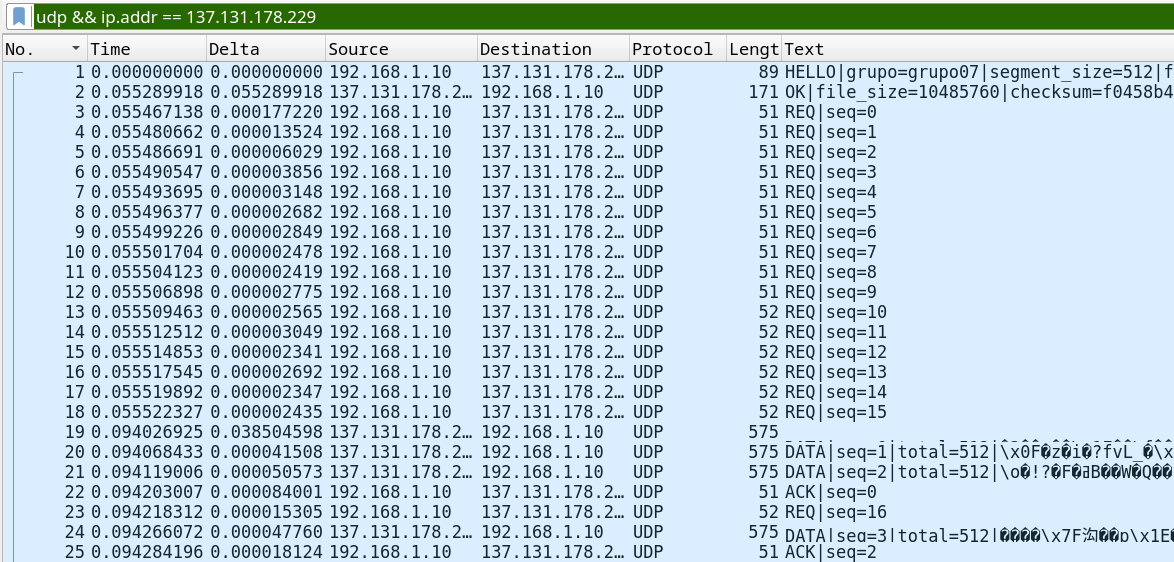
\includegraphics[width=0.85\linewidth]{../imgs/wireshark/e3_inicio.png}
    \caption{Início: \texttt{HELLO} (frame 1), \texttt{OK} com o MD5 (frame 2),
      os 16 \texttt{REQ}s da primeira janela (frames 3--18) e os primeiros
      \texttt{DATA}; o frame 19 é o \texttt{DATA|seq=0}.}
  \end{subfigure}

  \medskip
  \begin{subfigure}[t]{\linewidth}
    \centering
    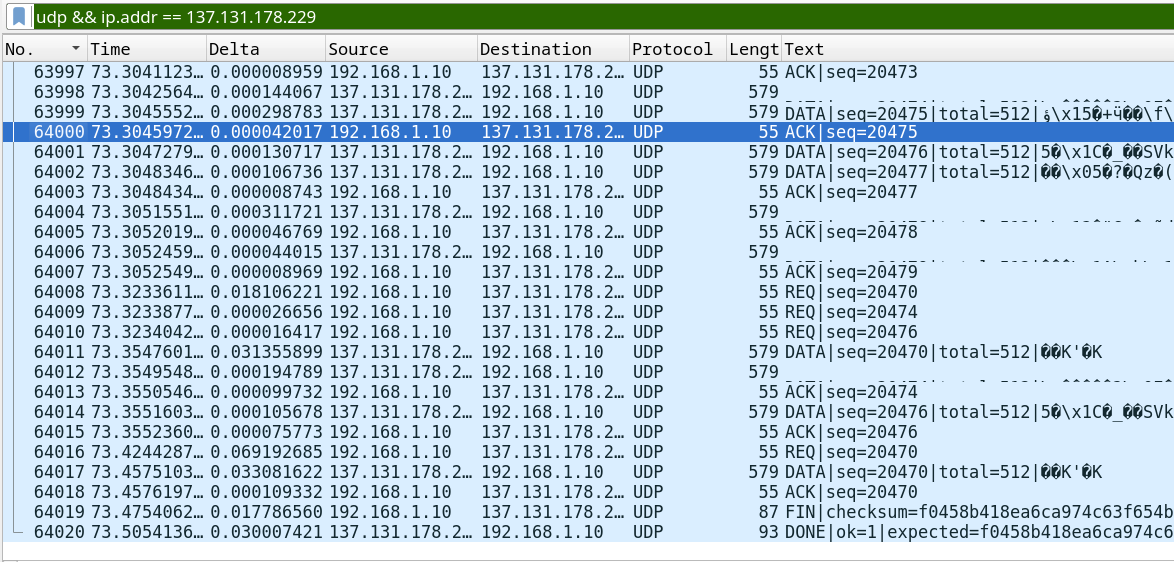
\includegraphics[width=0.85\linewidth]{../imgs/wireshark/e3_fim.png}
    \caption{Fim: últimos \texttt{DATA}/\texttt{ACK}, \texttt{FIN} com o MD5
      calculado (frame 64\,019, $t=73{,}475$\,s) e \texttt{DONE|ok=1}
      (frame 64\,020).}
  \end{subfigure}
  \caption{Sessão completa: \texttt{HELLO} $\rightarrow$ \texttt{REQ}s
    $\rightarrow$ \texttt{FIN} $\rightarrow$ \texttt{DONE}.}
  \label{fig:ws1}
\end{figure}

No fim (Figura~\ref{fig:ws1}b) aparecem \texttt{REQ}s repetidos dos segmentos
20\,470, 20\,474 e 20\,476: são as últimas perdas simuladas, reenviadas antes
do \texttt{FIN}.

\subsection{Eventos de retransmissão}

A captura tem 1\,234 segmentos com \texttt{REQ} repetido, os mesmos 1\,234 que
o CSV marca com \texttt{retransmissions} $\geq 1$. A Figura~\ref{fig:ws2}
mostra dois eventos com causas diferentes. Em cada um, o \texttt{REQ} original
foi marcado como referência de tempo (\texttt{*REF*}), então a coluna Time dá
o delta até os pacotes seguintes.

\begin{figure}[H]
  \centering
  \begin{subfigure}[t]{\linewidth}
    \centering
    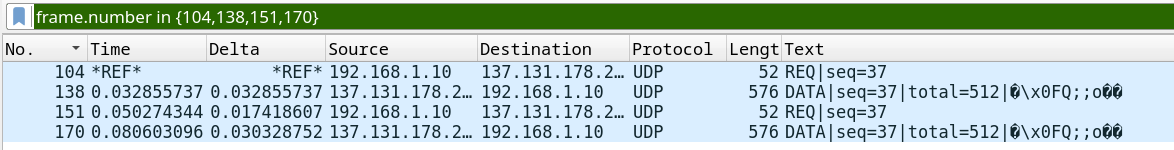
\includegraphics[width=0.85\linewidth]{../imgs/wireshark/e3_retx_perda.png}
    \caption{Segmento 37, perda simulada: o \texttt{DATA} do frame 138 chega
      em 32,9\,ms e é descartado pelo cliente; o \texttt{REQ} é repetido em
      50,3\,ms (frame 151) e o novo \texttt{DATA} chega em 80,6\,ms
      (frame 170).}
  \end{subfigure}

  \medskip
  \begin{subfigure}[t]{\linewidth}
    \centering
    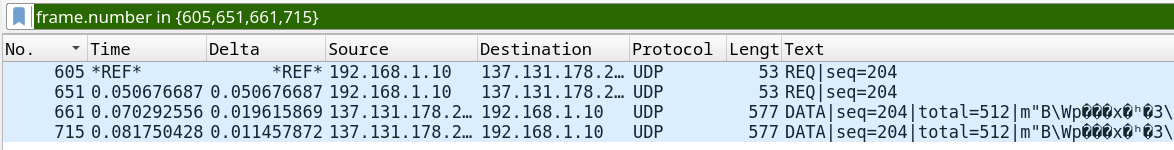
\includegraphics[width=0.85\linewidth]{../imgs/wireshark/e3_retx_atraso.png}
    \caption{Segmento 204, retransmissão desnecessária: o \texttt{REQ} é
      repetido em 50,7\,ms (frame 651), o \texttt{DATA} original chega em
      70,3\,ms (frame 661) e o duplicado em 81,8\,ms (frame 715).}
  \end{subfigure}
  \caption{Dois eventos de retransmissão, com o delta entre o \texttt{REQ}
    original e o retransmitido.}
  \label{fig:ws2}
\end{figure}

Nos dois casos o \texttt{REQ} foi repetido $\sim$50\,ms depois do original,
que é o piso do timeout. No segmento 37 a retransmissão era necessária: o
cliente descartou o primeiro \texttt{DATA}. No segmento 204 não era: o
\texttt{DATA} original levou 70,3\,ms, durante um bloco lento, e chegou 19,6\,ms
depois da retransmissão. O cliente reconheceu o caso pelo \texttt{DATA}
duplicado e usou os 70,3\,ms como amostra de RTT.

\subsection{Correlação com o CSV}

\begin{figure}[H]
  \centering
  \begin{subfigure}[t]{\linewidth}
    \centering
    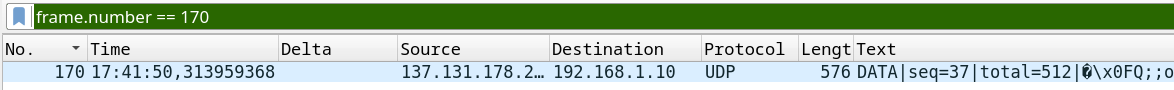
\includegraphics[width=0.85\linewidth]{../imgs/wireshark/e3_correlacao.png}
    \caption{Frame 170 (\texttt{DATA|seq=37} aceito) com o horário de chegada.}
  \end{subfigure}

  \medskip
  \begin{subfigure}[t]{\linewidth}
    \centering
    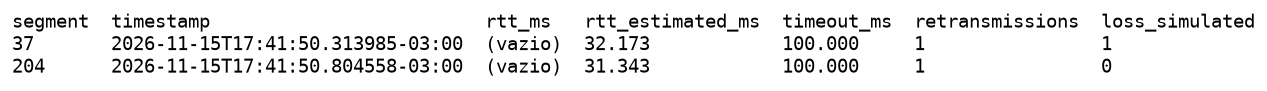
\includegraphics[width=\linewidth]{../imgs/wireshark/e3_csv_linhas.png}
    \caption{Linhas do CSV dos segmentos 37 e 204.}
  \end{subfigure}
  \caption{Correlação entre a captura e o CSV.}
  \label{fig:ws3}
\end{figure}

O \texttt{timestamp} do CSV é o instante em que o cliente aceitou o
\texttt{DATA}. O frame 170 chegou às 17:41:50,313959, e a linha do segmento 37
marca 17:41:50,313985, 0,026\,ms depois. O segmento 204 bate do mesmo jeito:
frame 661 às 17:41:50,804496 e CSV às 17:41:50,804558. Os outros campos
contam a mesma história da captura:
\begin{itemize}[nosep]
  \item \texttt{retransmissions=1} nos dois, e \texttt{loss\_simulated=1} só
    no 37, o único cujo \texttt{DATA} o cliente descartou;
  \item \texttt{rtt\_ms} vazio nos dois, porque segmentos retransmitidos não
    geram amostra direta;
  \item \texttt{timeout\_ms=100}: o timer do segmento dobrou de 50 para
    100\,ms com a retransmissão.
\end{itemize}

\subsection{Medição de RTT}

\figura{../imgs/wireshark/e3_rtt.png}{0.85\linewidth}{RTT do segmento~0:
\texttt{REQ|seq=0} (frame 3, referência) e \texttt{DATA|seq=0} (frame 19),
38,560\,ms depois.}{fig:ws4}

\begin{table}[H]
\centering\small
\begin{tabular}{lrrr}
\toprule
Segmento & RTT Wireshark (ms) & RTT CSV (ms) & Diferença (ms) \\
\midrule
0       & 38,560 & 38,697 & 0,137 \\
5\,000  & 32,194 & 32,200 & 0,006 \\
10\,000 & 33,696 & 33,701 & 0,005 \\
20\,479 & 32,847 & 32,852 & 0,005 \\
\midrule
19\,246 segmentos (mediana) & 31,950 & 31,968 & 0,022 (média) \\
\bottomrule
\end{tabular}
\caption{RTT medido no Wireshark (\texttt{REQ} $\rightarrow$ \texttt{DATA}) e
registrado pelo cliente. A última linha cobre todos os segmentos sem
retransmissão.}
\label{tab:ws-rtt}
\end{table}

Os valores são próximos. O cliente mede em média 0,022\,ms a mais que o
Wireshark, o tempo entre o pacote passar pela placa de rede e o Python ler o
socket. O segmento~0 tem a maior diferença (0,137\,ms) porque é o primeiro
pacote processado pelo cliente. Para o estimador, esse erro é desprezível
diante da variação do próprio RTT (33 a 65\,ms).

% ======================= 5 ===========================================
\section{Visão integrada: comparação final de todos os protocolos}

A Tabela~\ref{tab:final} reúne o melhor cenário de cada protocolo: arquivo
\emph{large}, sem perda simulada, $N=1$ no SAW e $N=16$ no GBN e no SR, todos
com timeout fixo de 1000\,ms ou adaptativo. O throughput é o arquivo inteiro
($\times 8$) dividido pelo tempo entre o primeiro \texttt{REQ} e o último
\texttt{DATA}. O timeout adaptativo foi implementado só no SR, como permite o
enunciado; por isso a linha do GBN adaptativo fica vazia.

\begin{table}[H]
\centering\small
\begin{tabular}{lrlrrr}
\toprule
Protocolo & Janela & Timeout & Throughput (kbit/s) & Retransmissões & Tempo total (s) \\
\midrule
SAW & 1  & fixo       & 140,9    & 0      & 595,3 \\
GBN & 16 & fixo       & 1\,838,5 & 48     & 45,6 \\
GBN & 16 & adaptativo & ---      & ---    & --- \\
SR  & 16 & fixo       & 1\,694,2 & 0      & 49,5 \\
SR  & 16 & adaptativo & 1\,482,5 & 1\,840 & 56,6 \\
\bottomrule
\end{tabular}
\caption{Visão integrada (arquivo \emph{large}, sem perda simulada). Com
perda, a comparação do SR está na Tabela~\ref{tab:fixo}.}
\label{tab:final}
\end{table}

\figura{../imgs/comparacao_throughput.png}{0.8\linewidth}{Throughput médio dos
protocolos da Tabela~\ref{tab:final}.}{fig:barras}

A janela é o que muda o desempenho. Sem perda, um protocolo com $N$
segmentos em voo envia no máximo $N \cdot L$ bits por RTT
(Kurose~\cite{kurose}, Seção~3.4), porque o tempo de transmissão de 512\,B é
desprezível perto do RTT. Com o RTT médio de cada execução, o SAW deveria ter
141,0\,kbit/s e mediu 140,9; o SR fixo deveria ter 1\,695,8 e mediu 1\,694,2.
Nas janelas da Entrega~2 a conta também fecha: com $N=4$, 8 e 16, o SR mediu
342,4, 1\,211,9 e 2\,000,6\,kbit/s, contra 342,6, 1\,214,6 e 2\,009,0
previstos. GBN e SR ficam de 10 a 13 vezes acima do SAW e terminam o arquivo em
menos de um minuto, contra quase dez.

Dois resultados se afastam da teoria. O GBN mediu 1\,838,5\,kbit/s, abaixo dos
1\,967,2 previstos, porque teve 3 timeouts de 1\,s causados por perdas reais
da rede; cada um reenviou a janela de 16 (as 48 retransmissões). Descontando
esses 3\,s, a previsão cai para 1\,838. Além disso, sem perda GBN e SR
deveriam empatar, mas o GBN ficou 8\% acima do SR fixo. A diferença é da rede:
o RTT médio foi de 33,3\,ms na execução do GBN e de 38,6\,ms na do SR, que pegou
mais blocos lentos. O SR adaptativo ficou abaixo dos dois pelas retransmissões
desnecessárias da Seção~\ref{sec:piso} e por um RTT médio ainda maior
(42,1\,ms).

A diferença entre os protocolos aparece com perda. Na Entrega~2, com 10\% de
perda, o GBN fez 920, 1\,840 e 3\,556 retransmissões com $N=4$, 8 e 16, e o
SR fez 220 em todos os casos. A razão (4,2, 8,4 e 16,2) acompanha $N$, como
esperado de um protocolo que reenvia a janela inteira a cada timeout.

% ======================= 6 ===========================================
\section{Conclusão}

No ambiente do projeto (rede real, RTT mediano de 29 a 34\,ms na campanha,
acima dos $\sim$22\,ms citados no enunciado), o SR com
$N=16$ e timeout adaptativo foi o melhor protocolo. Sem perda, GBN e SR com a
mesma janela empatam, porque quase não há o que retransmitir. Com perda, o SR
reenvia só o segmento atrasado, enquanto o GBN reenvia a janela: com 10\% de
perda, 220 retransmissões contra 3\,556, e 104\,s contra 226\,s no
\emph{small}. O timeout adaptativo completa o ganho: com 10\% de perda, o
SR transferiu os 10\,MB em 101\,s, contra 1\,042\,s com timeout fixo.

O RTT adaptativo valeu a complexidade, com uma ressalva. A fórmula do TCP
sozinha piorou o cliente: sem piso, o timeout colado no RTT gerou mais de mil
retransmissões desnecessárias numa transferência sem perda. Com o piso e o
backoff, o adaptativo reduziu o tempo em cerca de 10 vezes com 5\% e 10\% de
perda. O custo ficou nas transferências sem perda, em que ele foi 14\% mais
lento que o fixo por causa dos blocos lentos da rede.

Se fôssemos recomeçar, faríamos três coisas de outro jeito:
\begin{itemize}[nosep]
  \item Rodar todos os experimentos numa campanha única e automatizada desde a
    primeira entrega, guardando o log com o MD5 de cada execução. Foi o que
    fizemos para este relatório, depois de comparações entre execuções de dias
    diferentes terem medido mais a rede que o protocolo.
  \item Escrever o estimador de RTT junto com a reprodução de traços antes de
    ir à rede real. A reprodução comparou $\alpha$ e $\beta$ com os mesmos
    dados, o que as execuções reais não conseguem.
  \item Implementar o timeout adaptativo num módulo de temporização comum aos
    três protocolos, e não só no SR.
\end{itemize}

% ======================= ANEXOS ======================================
\section*{Anexos}
\addcontentsline{toc}{section}{Anexos}
\begin{sloppypar}

\textbf{Código e CSVs.} O código-fonte e os CSVs de todas as execuções estão
no repositório do grupo, \url{https://github.com/luricl/RDT-UnB}. Os 42 CSVs da
campanha seguem o padrão
\texttt{metrics\_grupo07\_<protocolo>\_<AAAAMMDD\_HHMMSS>.csv} e ficam em
\texttt{results/final/csv}. O arquivo \texttt{results/final/execucoes.csv}
liga cada cenário ao seu CSV, e \texttt{results/final/logs} guarda a saída do
cliente de cada execução. A captura do Wireshark está em
\texttt{results/final/captura}.

\textbf{MD5.} Todas as execuções terminaram com o MD5 calculado igual ao
\texttt{checksum} do \texttt{OK} e com \texttt{DONE|ok=1}:
\begin{itemize}[nosep]
  \item small (1\,048\,576 bytes, 21 execuções):
    \texttt{f082218dabf5c0296ab90d12d90b170a};
  \item medium (5\,242\,880 bytes, 1 execução):
    \texttt{ff79a3ea02665142b2f27746cfe3da30};
  \item large (10\,485\,760 bytes, 20 execuções):
    \texttt{f0458b418ea6ca974c63f654baee06fc}.
\end{itemize}

\end{sloppypar}

% ======================= REFERÊNCIAS =================================
\begin{thebibliography}{9}
  \bibitem{kurose} J. F. Kurose e K. W. Ross, \textit{Computer Networking: A Top-Down
    Approach}, 8th ed. Hoboken: Pearson, 2021.
  \bibitem{rfc768} J. Postel, ``User Datagram Protocol,'' RFC 768, IETF, 1980.
    Disponível em: \url{https://www.rfc-editor.org/rfc/rfc768}.
  \bibitem{rfc1321} R. Rivest, ``The MD5 Message-Digest Algorithm,'' RFC 1321, IETF, 1992.
    Disponível em: \url{https://www.rfc-editor.org/rfc/rfc1321}.
\end{thebibliography}

\end{document}
